\documentclass[11pt]{amsart}
\usepackage{geometry}                % See geometry.pdf to learn the layout options. There are lots.
\geometry{letterpaper}                   % ... or a4paper or a5paper or ... 
%\geometry{landscape}                % Activate for for rotated page geometry
%\usepackage[parfill]{parskip}    % Activate to begin paragraphs with an empty line rather than an indent
\usepackage{graphicx}
\usepackage{amssymb}
\usepackage{epstopdf}
\usepackage{color}
\usepackage{hyperref}

\DeclareGraphicsRule{.tif}{png}{.png}{`convert #1 `dirname #1`/`basename #1 .tif`.png}

\title{Brief Article}
\author{The Author}
%\date{}                                           % Activate to display a given date or no date

\begin{document}
%\maketitle
\section{Variant on pythagorean triples}
%\subsection{}

(followed up and generalised on stack exchange, see later sections)

In [Weissman, Illustrated Theory of Numbers (AMS)], there is a nice description of how to generate a mapping between reduced fractions and pythagorean triples.
In outline the method is as follows:

Take the unit circle $x^2+y^2=1$ and a straight line through $(0,1)$ with a rational gradient $m$, i.e. $y = mx + 1$ (see picture).

The  line  and the circle intersect at $(0,1)$ and $(u,v)$. The coordinates of the second point can be found to be 
$$
u = \frac{- 2 m}{{{m}^{2}}+1} \qquad 
\text{ and }
\qquad
v = \frac{{ - {m}^{2}} + 1}{{{m}^{2}}+1}
$$

As $m$ is rational, we can write it as $a/b$ with gcd$(a,b)=1$ and we can re-write $u$ and $v$.
$$
u = -\frac{2 a b}{{{b}^{2}}+{{a}^{2}}}
\qquad 
\text{ and }
\qquad
v = \frac{{{b}^{2}}-{{a}^{2}}}{{{b}^{2}}+{{a}^{2}}}
$$

Using the fact that $u^2+v^2 = 1$ leads to
$$
(2ab)^2 + (b^2-a^2)^2 = (b^2 + a^2)^2
$$
which gives a pythagorean triple $2ab$, $b^2-a^2$ and $a^2+b^2$. It is possible to show that only 1 is a common divisor for the triple.

Subsequently, there is an exercise to show that there are an infinite number of triples $(x,y,z)$ of the form $x^2 + 2 y^2 = 3 z^2$.

The hint is to use the point $(1,1)$ instead of the point $(0,1)$ for the line in a similar argument to that given above, i.e. to use the line $y = m(x-1) + 1$.

When I do this, still using the unit circle, I get quite complex expressions for the intersection coordinates. For example, one intersection point has
\[u = \frac{{{m}^{2}} - m -  \sqrt{2m}}{{{m}^{2}}+1}\]
Substituting in an expression for a reduced fraction makes things even more complicated and I cannot link the expressions for $u$ and $v$ to a triple of the form described.

Any advice on how I might proceed would be gratefully received.

\begin{center}
\includegraphics[width=0.3\textwidth]{pics/pythag-triples}
\end{center}

\section{After feedback from maths stack exchange.}

\href{https://math.stackexchange.com/questions/2601414/variant-of-pythagorean-triples}{Link ...}


Show that it is possible to generate pythagorean type triples $(x,y,z)$ such that $x^2 + 2 y^2 = z^2$.  Proceed by looking at the intersection of lines through $(1,1)$ and the ellipse $x^2 + 2 y^2 = 3$. The point $(1,1)$ is on the ellipse. The second intersection is at $(u,v)$ which depends on $m$ (the gradient of the line).  Writing $m = a/b$ gives expressions for $x$, $y$ and $z$ 


\noindent
%%%%%%%%%%%%%%%
%%% INPUT:
\begin{minipage}[t]{8ex}\color{red}\bf
(\%{}i16) 
\end{minipage}
\begin{minipage}[t]{\textwidth}\color{blue}
ya : 1 + m*(x-1);
\end{minipage}
%%% OUTPUT:
\[\displaystyle
\tag{ya}\label{ya}
m\,\left( x-1\right) +1\mbox{}
\]
%%%%%%%%%%%%%%%



\noindent
%%%%%%%%%%%%%%%
%%% INPUT:
\begin{minipage}[t]{8ex}\color{red}\bf
(\%{}i25) 
\end{minipage}
\begin{minipage}[t]{\textwidth}\color{blue}
crossings: solve([2*ya\^{}2 + x\^{}2 = 3], [x]);
\end{minipage}
%%% OUTPUT:
\[\displaystyle
\tag{crossings}\label{crossings}
[x=\frac{2{{m}^{2}}-4m-1}{2{{m}^{2}}+1},x=1]\mbox{}
\]
%%%%%%%%%%%%%%%


\noindent
%%%%%%%%%%%%%%%
%%% INPUT:
\begin{minipage}[t]{8ex}\color{red}\bf
(\%{}i26) 
\end{minipage}
\begin{minipage}[t]{\textwidth}\color{blue}
u: crossings[1];
\end{minipage}
%%% OUTPUT:
\[\displaystyle
\tag{u}\label{u}
x=\frac{2{{m}^{2}}-4m-1}{2{{m}^{2}}+1}\mbox{}
\]
%%%%%%%%%%%%%%%


\noindent
%%%%%%%%%%%%%%%
%%% INPUT:
\begin{minipage}[t]{8ex}\color{red}\bf
(\%{}i28) 
\end{minipage}
\begin{minipage}[t]{\textwidth}\color{blue}
v: ratsimp(m*(u-1) + 1);
\end{minipage}
%%% OUTPUT:
\[\displaystyle
\tag{v}\label{v}
mx-m+1=-\frac{2{{m}^{2}}+2m-1}{2{{m}^{2}}+1}\mbox{}
\]
%%%%%%%%%%%%%%%


\noindent
%%%%%%%%%%%%%%%
%%% INPUT:
\begin{minipage}[t]{8ex}\color{red}\bf
(\%{}i29) 
\end{minipage}
\begin{minipage}[t]{\textwidth}\color{blue}
ratsimp(u\^{}2);
\end{minipage}
%%% OUTPUT:
\[\displaystyle
\tag{\%{}o29}\label{o29} 
{{x}^{2}}=\frac{4{{m}^{4}}-16{{m}^{3}}+12{{m}^{2}}+8m+1}{4{{m}^{4}}+4{{m}^{2}}+1}\mbox{}
\]
%%%%%%%%%%%%%%%


\noindent
%%%%%%%%%%%%%%%
%%% INPUT:
\begin{minipage}[t]{8ex}\color{red}\bf
(\%{}i30) 
\end{minipage}
\begin{minipage}[t]{\textwidth}\color{blue}
ratsimp(v\^{}2);
\end{minipage}
%%% OUTPUT:
\[\displaystyle
\tag{\%{}o30}\label{o30} 
{{m}^{2}}\,{{x}^{2}}+\left( 2m-2{{m}^{2}}\right) x+{{m}^{2}}-2m+1=\frac{4{{m}^{4}}+8{{m}^{3}}-4m+1}{4{{m}^{4}}+4{{m}^{2}}+1}\mbox{}
\]
%%%%%%%%%%%%%%%


\noindent
%%%%%%%%%%%%%%%
%%% INPUT:
\begin{minipage}[t]{8ex}\color{red}\bf
(\%{}i44) 
\end{minipage}
\begin{minipage}[t]{\textwidth}\color{blue}
ratsimp(u\^{}2 + 2*v\^{}2);
\end{minipage}
%%% OUTPUT:
\[\displaystyle
\tag{\%{}o44}\label{o44} 
\left( 2{{m}^{2}}+1\right) \,{{x}^{2}}+\left( 4m-4{{m}^{2}}\right) x+2{{m}^{2}}-4m+2=3\mbox{}
\]
%%%%%%%%%%%%%%%


\noindent
%%%%%%%%%%%%%%%
%%% INPUT:
\begin{minipage}[t]{8ex}\color{red}\bf
(\%{}i32) 
\end{minipage}
\begin{minipage}[t]{\textwidth}\color{blue}
ratsimp(subst(m = a/b, u));
\end{minipage}
%%% OUTPUT:
\[\displaystyle
\tag{\%{}o32}\label{o32} 
x=-\frac{{{b}^{2}}+4ab-2{{a}^{2}}}{{{b}^{2}}+2{{a}^{2}}}\mbox{}
\]
%%%%%%%%%%%%%%%


\noindent
%%%%%%%%%%%%%%%
%%% INPUT:
\begin{minipage}[t]{8ex}\color{red}\bf
(\%{}i33) 
\end{minipage}
\begin{minipage}[t]{\textwidth}\color{blue}
ratsimp(subst(m = a/b, v));
\end{minipage}
%%% OUTPUT:
\[\displaystyle
\tag{\%{}o33}\label{o33} 
\frac{ax+b-a}{b}=\frac{{{b}^{2}}-2ab-2{{a}^{2}}}{{{b}^{2}}+2{{a}^{2}}}\mbox{}
\]
%%%%%%%%%%%%%%%


\noindent
%%%%%%%%%%%%%%%
%%% INPUT:
\begin{minipage}[t]{8ex}\color{red}\bf
(\%{}i45) 
\end{minipage}
\begin{minipage}[t]{\textwidth}\color{blue}
X: 2*a\^{}2 - 4*a*b - b\^{}2;
\end{minipage}
%%% OUTPUT:
\[\displaystyle
\tag{X}\label{X}
-{{b}^{2}}-4ab+2{{a}^{2}}\mbox{}
\]
%%%%%%%%%%%%%%%


\noindent
%%%%%%%%%%%%%%%
%%% INPUT:
\begin{minipage}[t]{8ex}\color{red}\bf
(\%{}i46) 
\end{minipage}
\begin{minipage}[t]{\textwidth}\color{blue}
Y: b\^{}2-2*a*b-2*a\^{}2;
\end{minipage}
%%% OUTPUT:
\[\displaystyle
\tag{Y}\label{Y}
{{b}^{2}}-2ab-2{{a}^{2}}\mbox{}
\]
%%%%%%%%%%%%%%%


\noindent
%%%%%%%%%%%%%%%
%%% INPUT:
\begin{minipage}[t]{8ex}\color{red}\bf
(\%{}i47) 
\end{minipage}
\begin{minipage}[t]{\textwidth}\color{blue}
Z: b\^{}2+2*a\^{}2;
\end{minipage}
%%% OUTPUT:
\[\displaystyle
\tag{Z}\label{Z}
{{b}^{2}}+2{{a}^{2}}\mbox{}
\]
%%%%%%%%%%%%%%%


\noindent
%%%%%%%%%%%%%%%
%%% INPUT:
\begin{minipage}[t]{8ex}\color{red}\bf
(\%{}i48) 
\end{minipage}
\begin{minipage}[t]{\textwidth}\color{blue}
ratsimp(X\^{}2 + 2*Y\^{}2);
\end{minipage}
%%% OUTPUT:
\[\displaystyle
\tag{\%{}o48}\label{o48} 
3{{b}^{4}}+12{{a}^{2}}\,{{b}^{2}}+12{{a}^{4}}\mbox{}
\]
%%%%%%%%%%%%%%%


\noindent
%%%%%%%%%%%%%%%
%%% INPUT:
\begin{minipage}[t]{8ex}\color{red}\bf
(\%{}i50) 
\end{minipage}
\begin{minipage}[t]{\textwidth}\color{blue}
ratsimp(3*Z\^{}2);
\end{minipage}
%%% OUTPUT:
\[\displaystyle
\tag{\%{}o50}\label{o50} 
3{{b}^{4}}+12{{a}^{2}}\,{{b}^{2}}+12{{a}^{4}}\mbox{}
\]
%%%%%%%%%%%%%%%


\noindent
%%%%%%%%%%%%%%%
%%% INPUT:
\begin{minipage}[t]{8ex}\color{red}\bf
(\%{}i23) 
\end{minipage}
\begin{minipage}[t]{\textwidth}\color{blue}
wxplot2d([sqrt((3 - x\^{}2)/2), -sqrt((3 - x\^{}2)/2)], [x,-3,3],
 [gnuplot\_postamble, "set zeroaxis;"])\$
\end{minipage}
%%% OUTPUT:
\[\displaystyle
\mbox{}\\\mbox{plot2d: expression evaluates to non-numeric value somewhere in plotting range.}\mbox{}\\\mbox{plot2d: expression evaluates to non-numeric value somewhere in plotting range.}\mbox{}\]
\[\displaystyle
\]
\[\tag{\%{}t23}\label{t23} 
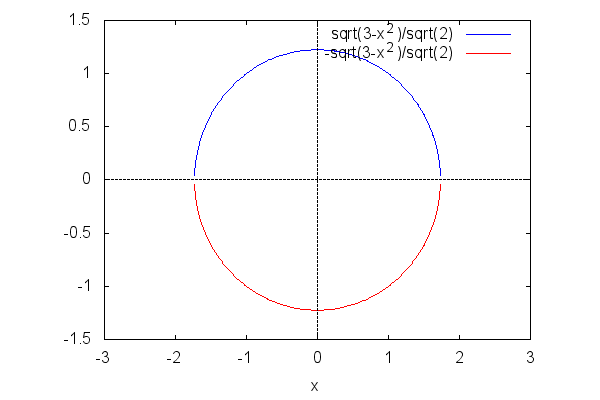
\includegraphics[width=.95\linewidth,height=.80\textheight,keepaspectratio]{pics/weissman_2_1}\mbox{}
\]
%%%%%%%%%%%%%%%

\section{Further generalisation with Maxima}


Find forms for $(x,y,z)$ that satisfy $2 x^{2} + 3 y^{2} = 5$ in terms of parameters $(a,b)$. Generalisation of pythagorean triples. 


\noindent
%%%%%%%%%%%%%%%
%%% INPUT:
\begin{minipage}[t]{8ex}\color{red}\bf
(\%{}i1) 
\end{minipage}
\begin{minipage}[t]{\textwidth}\color{blue}
ya : 1 + m*(x-1);
\end{minipage}
%%% OUTPUT:
\[\displaystyle
\tag{ya}\label{ya}
m\,\left( x-1\right) +1\mbox{}
\]
%%%%%%%%%%%%%%%


\noindent
%%%%%%%%%%%%%%%
%%% INPUT:
\begin{minipage}[t]{8ex}\color{red}\bf
(\%{}i2) 
\end{minipage}
\begin{minipage}[t]{\textwidth}\color{blue}
crossings: solve([3*ya\^{}2 + 2*x\^{}2 = 5], [x]);
\end{minipage}
%%% OUTPUT:
\[\displaystyle
\tag{crossings}\label{crossings}
[x=\frac{3{{m}^{2}}-6m-2}{3{{m}^{2}}+2},x=1]\mbox{}
\]
%%%%%%%%%%%%%%%


\noindent
%%%%%%%%%%%%%%%
%%% INPUT:
\begin{minipage}[t]{8ex}\color{red}\bf
(\%{}i3) 
\end{minipage}
\begin{minipage}[t]{\textwidth}\color{blue}
u: crossings[1];
\end{minipage}
%%% OUTPUT:
\[\displaystyle
\tag{u}\label{u}
x=\frac{3{{m}^{2}}-6m-2}{3{{m}^{2}}+2}\mbox{}
\]
%%%%%%%%%%%%%%%


\noindent
%%%%%%%%%%%%%%%
%%% INPUT:
\begin{minipage}[t]{8ex}\color{red}\bf
(\%{}i4) 
\end{minipage}
\begin{minipage}[t]{\textwidth}\color{blue}
v: ratsimp(m*(u-1) + 1);
\end{minipage}
%%% OUTPUT:
\[\displaystyle
\tag{v}\label{v}
mx-m+1=-\frac{3{{m}^{2}}+4m-2}{3{{m}^{2}}+2}\mbox{}
\]
%%%%%%%%%%%%%%%


\noindent
%%%%%%%%%%%%%%%
%%% INPUT:
\begin{minipage}[t]{8ex}\color{red}\bf
(\%{}i5) 
\end{minipage}
\begin{minipage}[t]{\textwidth}\color{blue}
ratsimp(subst(m = a/b, u));
\end{minipage}
%%% OUTPUT:
\[\displaystyle
\tag{\%{}o5}\label{o5} 
x=-\frac{2{{b}^{2}}+6ab-3{{a}^{2}}}{2{{b}^{2}}+3{{a}^{2}}}\mbox{}
\]
%%%%%%%%%%%%%%%


\noindent
%%%%%%%%%%%%%%%
%%% INPUT:
\begin{minipage}[t]{8ex}\color{red}\bf
(\%{}i6) 
\end{minipage}
\begin{minipage}[t]{\textwidth}\color{blue}
ratsimp(subst(m = a/b, v));
\end{minipage}
%%% OUTPUT:
\[\displaystyle
\tag{\%{}o6}\label{o6} 
\frac{ax+b-a}{b}=\frac{2{{b}^{2}}-4ab-3{{a}^{2}}}{2{{b}^{2}}+3{{a}^{2}}}\mbox{}
\]
%%%%%%%%%%%%%%%


\noindent
%%%%%%%%%%%%%%%
%%% INPUT:
\begin{minipage}[t]{8ex}\color{red}\bf
(\%{}i7) 
\end{minipage}
\begin{minipage}[t]{\textwidth}\color{blue}
X: 2*b\^{}2+6*a*b-3*a\^{}2;
\end{minipage}
%%% OUTPUT:
\[\displaystyle
\tag{X}\label{X}
2{{b}^{2}}+6ab-3{{a}^{2}}\mbox{}
\]
%%%%%%%%%%%%%%%


\noindent
%%%%%%%%%%%%%%%
%%% INPUT:
\begin{minipage}[t]{8ex}\color{red}\bf
(\%{}i8) 
\end{minipage}
\begin{minipage}[t]{\textwidth}\color{blue}
Y: 2*b\^{}2-4*a*b-3*a\^{}2;
\end{minipage}
%%% OUTPUT:
\[\displaystyle
\tag{Y}\label{Y}
2{{b}^{2}}-4ab-3{{a}^{2}}\mbox{}
\]
%%%%%%%%%%%%%%%


\noindent
%%%%%%%%%%%%%%%
%%% INPUT:
\begin{minipage}[t]{8ex}\color{red}\bf
(\%{}i9) 
\end{minipage}
\begin{minipage}[t]{\textwidth}\color{blue}
Z: 2*b\^{}2+3*a\^{}2;
\end{minipage}
%%% OUTPUT:
\[\displaystyle
\tag{Z}\label{Z}
2{{b}^{2}}+3{{a}^{2}}\mbox{}
\]
%%%%%%%%%%%%%%%


\noindent
%%%%%%%%%%%%%%%
%%% INPUT:
\begin{minipage}[t]{8ex}\color{red}\bf
(\%{}i10) 
\end{minipage}
\begin{minipage}[t]{\textwidth}\color{blue}
ratsimp(2*X\^{}2 + 3*Y\^{}2);
\end{minipage}
%%% OUTPUT:
\[\displaystyle
\tag{\%{}o10}\label{o10} 
20{{b}^{4}}+60{{a}^{2}}\,{{b}^{2}}+45{{a}^{4}}\mbox{}
\]
%%%%%%%%%%%%%%%


\noindent
%%%%%%%%%%%%%%%
%%% INPUT:
\begin{minipage}[t]{8ex}\color{red}\bf
(\%{}i11) 
\end{minipage}
\begin{minipage}[t]{\textwidth}\color{blue}
ratsimp(5*Z\^{}2);
\end{minipage}
%%% OUTPUT:
\[\displaystyle
\tag{\%{}o11}\label{o11} 
20{{b}^{4}}+60{{a}^{2}}\,{{b}^{2}}+45{{a}^{4}}\mbox{}
\]
%%%%%%%%%%%%%%%







































\end{document}  